% Gerado por ferramentas/importar_relatorios.py a partir de MLP/ARTIGO_SIM_EMBARCADO-10.11.2026/ARTIGO_SIM_EMBARCADO.tex.
% Revisado à mão na dissertação: edite este arquivo, não a fonte.
\subsection{Resultados}
\label{sim:sec:resultados}

\subsubsection{Fidelidade numérica da inferência (V0 e V1)}

A rede reconstruída em ponto flutuante a partir dos pesos exportados reproduziu o \texttt{scikit-learn} com diferença máxima de \(7\times10^{-13}\)\,Hz e classes idênticas. Em C, o caminho float32 ficou a no máximo \(2{,}5\times10^{-4}\)\,Hz do Python, com classes idênticas, e o caminho int8 reproduziu bit a bit os acumuladores e as classes da emulação inteira nas 3\,540 janelas.

A Figura~\ref{sim:fig:quantizacao} mostra o efeito da própria quantização, isto é, int8 contra float32. A diferença na frequência é pequena e centrada (média de \(-0{,}22\)\,Hz, \(|\Delta|\) médio de 0,81\,Hz, 95\,\% das janelas abaixo de 2,3\,Hz), com poucos casos isolados de até 11,8\,Hz. O nível de 10\,Hz arredondado coincide em 96,6\,\% das janelas e a classe de válvulas em 98,2\,\% (Tabela~\ref{sim:tab:fidelidade}). No próprio conjunto de treino, o erro médio da frequência passou de 1,54 para 1,81\,Hz e a acurácia das válvulas, de 92,8 para 92,5\,\%; em ambos os casos, a perda é muito menor que a diferença entre validação dentro e fora da corrida (Seção~\ref{sec:res_bomba}).

\begin{figure}[htbp]
	\centering
	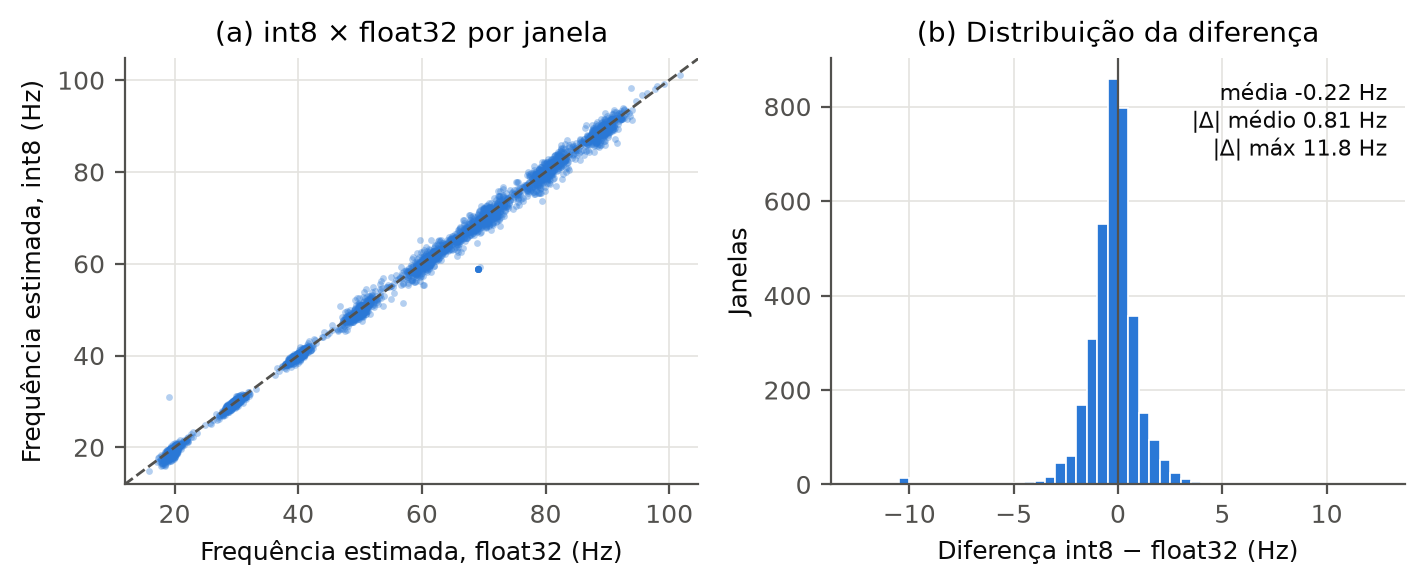
\includegraphics[width=\textwidth]{figs/embarcado/fig_quantizacao.png}
	\caption{Efeito da quantização int8 sobre a frequência estimada nas 3\,540 janelas: (a) estimativa int8 contra float32, com a reta identidade tracejada; (b) distribuição da diferença.}
	\label{sim:fig:quantizacao}
\end{figure}

\begin{table}[htbp]
	\centering
	\small
	\caption{Concordância entre implementações (3\,540 janelas). ``Nível'' é a frequência arredondada a 10\,Hz.}
	\label{sim:tab:fidelidade}
	\begin{tabular}{L{0.42\textwidth}ccc}
		\toprule
		\textbf{Comparação} & \textbf{Classe igual} & \textbf{Nível igual} & \textbf{\(|\Delta f|\) máx.} \\
		\midrule
		C float32 \(\times\) \texttt{scikit-learn} & 100\,\% & 100\,\% & \(2{,}5\times10^{-4}\)\,Hz \\
		C int8 \(\times\) emulação int8 (Python) & 100\,\% & 100\,\% & 0 (bit a bit) \\
		int8 \(\times\) float32 (efeito da quantização) & 98,2\,\% & 96,6\,\% & 11,8\,Hz \\
		Cadeia em C, percentis exatos \(\times\) Python int8 & 100\,\% & 100\,\% & 1,2\,Hz \\
		Cadeia em C, histograma \(\times\) Python int8 & 97,4\,\% & 96,2\,\% & 6,4\,Hz \\
		\bottomrule
	\end{tabular}
\end{table}

\subsubsection{Descritores e cadeia completa (V2)}

As fórmulas da Equação~\eqref{sim:eq:conversao}, aplicadas aos campos brutos, reproduziram as colunas físicas do \texttt{hits.csv} com erro relativo de no máximo \(10^{-5}\), compatível com o arredondamento do próprio arquivo. A Figura~\ref{sim:fig:descritores} mostra o erro normalizado máximo de cada descritor, nos dois canais, partindo do registro bruto. No modo exato, todos os erros ficaram abaixo de \(10^{-5}\), no nível da precisão simples; taxas e frações foram exatas, e os valores NaN coincidiram em todas as janelas. No modo histograma, os percentis ficaram acima da tolerância, como esperado de uma quantização em classes de largura fixa, com erros de até 0,2\,dB na amplitude, 0,04 nos logaritmos e 1,5\,kHz na frequência média.

\begin{figure}[htbp]
	\centering
	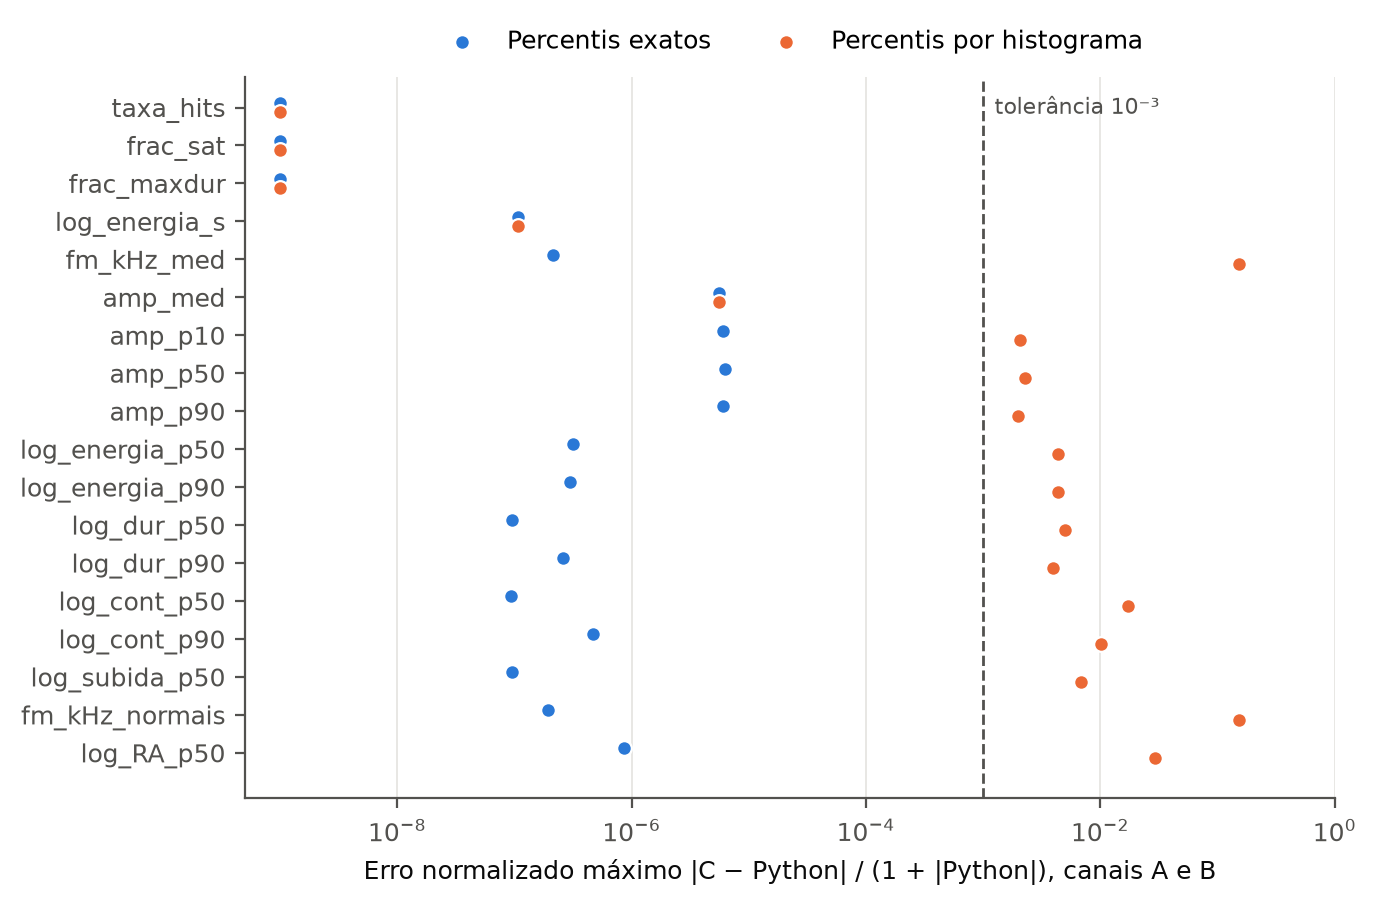
\includegraphics[width=0.92\textwidth]{figs/embarcado/fig_erro_descritores.png}
	\caption{Erro normalizado máximo, \(|x_{\mathrm{C}} - x_{\mathrm{Py}}|/(1+|x_{\mathrm{Py}}|)\), de cada descritor calculado em C a partir do registro bruto, nos dois modos de percentis, sobre as 3\,540 janelas e os dois canais. Erros nulos são desenhados em \(10^{-9}\). A linha tracejada é a tolerância de \(10^{-3}\).}
	\label{sim:fig:descritores}
\end{figure}

O que importa para a aplicação é a saída das redes. Com percentis exatos, a cadeia completa em C devolveu a mesma classe e o mesmo nível de frequência que o Python em 100\,\% das janelas; a maior diferença de frequência, 1,2\,Hz, vem do arredondamento da amplitude no \texttt{hits.csv}, que o C não usa ao partir do registro bruto. Com histogramas, a classe coincidiu em 97,4\,\% e o nível em 96,2\,\% (Tabela~\ref{sim:tab:fidelidade}), uma perda comparável à da própria quantização.

\subsubsection{Núcleo em lógica dedicada (V3 e V4)}

A simulação C e a cossimulação C/RTL do núcleo HLS, com 256 janelas, terminaram sem nenhuma divergência nos acumuladores ou na classe. A latência das duas redes foi de 11\,391 ciclos na síntese e de 11\,268 a 11\,393 ciclos na cossimulação, ou cerca de 114\,\(\mu\)s a 100\,MHz. Cada neurônio custa o número de entradas mais cerca de 12 ciclos de enchimento do \textit{pipeline}.

A Tabela~\ref{sim:tab:recursos} compara a estimativa da síntese HLS com o resultado após posicionamento e roteamento fora de contexto. A temporização foi atendida com folga: o caminho crítico tem 6,84\,ns, o que admitiria cerca de 146\,MHz. A implementação ocupou bem menos LUTs que a estimativa (656 contra 2\,421), porque a síntese lógica absorve parte da lógica de controle, e mais DSPs (14 contra 10), por causa da multiplicação de 64 bits da requantização. Os 3,5 blocos de BRAM guardam os 8\,960 pesos int8 das duas redes.

\begin{table}[htbp]
	\centering
	\small
	\caption{Recursos do IP HLS no XC7A35T (100\,MHz).}
	\label{sim:tab:recursos}
	\begin{tabular}{lrrrr}
		\toprule
		\textbf{Recurso} & \textbf{Estimativa HLS} & \textbf{Pós-roteamento} & \textbf{Disponível} & \textbf{Uso} \\
		\midrule
		LUT & 2\,421 & 656 & 20\,800 & 3,2\,\% \\
		\textit{Flip-flops} & 1\,648 & 682 & 41\,600 & 1,6\,\% \\
		DSP48E1 & 10 & 14 & 90 & 15,6\,\% \\
		BRAM (blocos de 36\,kb) & 3,5 & 3,5 & 50 & 7,0\,\% \\
		Período (ns) & 7,00 & 6,84 & 10,00 (alvo) & --- \\
		\bottomrule
	\end{tabular}
\end{table}

\subsubsection{Programa na MicroBlaze (V5)}

As seis simulações RTL (três programas \(\times\) duas configurações do processador) terminaram com a mesma sequência de valores de resultado da execução no computador: mesmas classes, mesmos acumuladores e, no modo exato, nenhum descritor fora da tolerância. Isso confirma, no nível do processador, que o binário embarcado reproduz o modelo. A Tabela~\ref{sim:tab:ciclos} resume os ciclos medidos.

\begin{table}[htbp]
	\centering
	\small
	\caption{Ciclos medidos na simulação RTL da MicroBlaze (100\,MHz, memória local, sem caches). Com FPU, médias sobre 2 vetores (MLP) e 2 janelas reais com 163 \textit{hits} (cadeia); sem FPU, 1 vetor e 1 janela com 81 \textit{hits}.}
	\label{sim:tab:ciclos}
	\begin{tabular}{lrr}
		\toprule
		\textbf{Etapa} & \textbf{Sem FPU} & \textbf{Com FPU} \\
		\midrule
		MLP float32, duas redes & \mbMlpFloatSoft & \mbMlpFloatFpu \\
		Quantização da entrada & \mbQuantSoft & \mbQuantFpu \\
		Núcleo int8, duas redes & \mbMlpIntSoft & \mbMlpIntFpu \\
		Inferência int8 completa (\(\mu\)s) & \mbMlpIntSoftUs & \mbMlpIntFpuUs \\
		\midrule
		Por \textit{hit}, modo exato & \mbHitSoft & \mbHitFpu \\
		Por \textit{hit}, modo histograma & \mbHitHistSoft & \mbHitHistFpu \\
		Fechar a janela, modo exato & \mbFecharSoft & \mbFecharFpu \\
		Fechar a janela, modo histograma & \mbFecharHistSoft & \mbFecharHistFpu \\
		\bottomrule
	\end{tabular}
\end{table}

\mbParagrafoMlp

A Figura~\ref{sim:fig:latencia} compara a latência da inferência nas plataformas. A Figura~\ref{sim:fig:ciclosjanela} decompõe o custo de uma janela típica dos dados (cerca de 80 \textit{hits}), e a Figura~\ref{sim:fig:carga} extrapola, a partir dos ciclos medidos, a ocupação da CPU em função da taxa de \textit{hits}.

\begin{figure}[htbp]
	\centering
	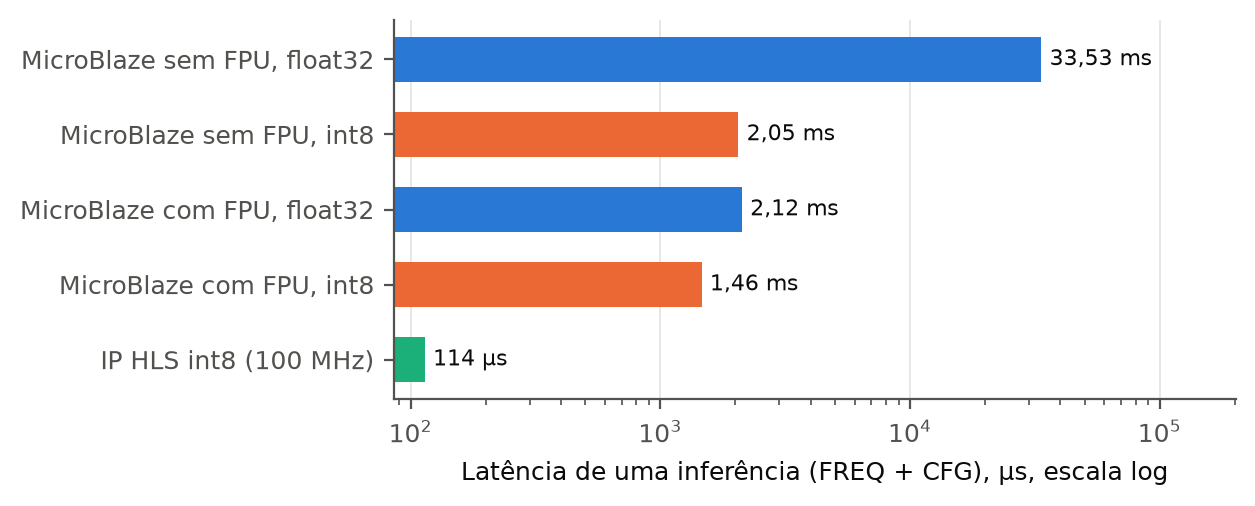
\includegraphics[width=0.85\textwidth]{figs/embarcado/fig_latencia_mlp.png}
	\caption{Latência de uma inferência (regressor e classificador) na MicroBlaze, medida em simulação RTL, e no IP HLS, medida na cossimulação. A MicroBlaze int8 inclui a quantização da entrada.}
	\label{sim:fig:latencia}
\end{figure}

\begin{figure}[htbp]
	\centering
	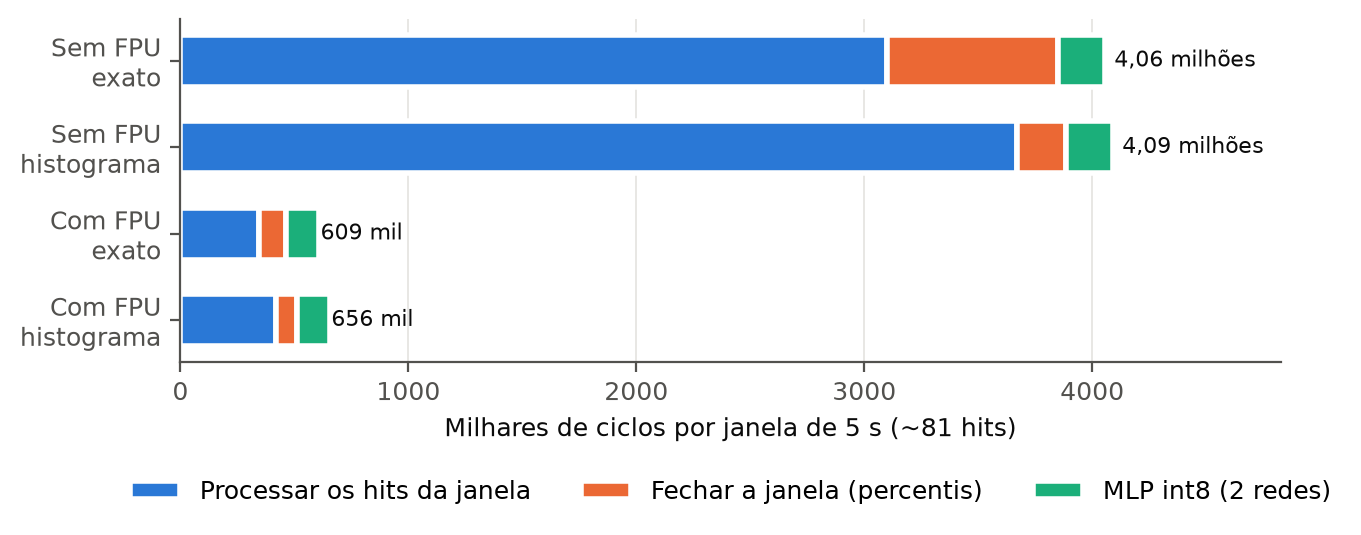
\includegraphics[width=0.92\textwidth]{figs/embarcado/fig_ciclos_janela.png}
	\caption{Composição dos ciclos de uma janela de 5\,s na MicroBlaze, para uma janela real de 81 \textit{hits} (custos por \textit{hit} medidos): processamento dos \textit{hits}, fechamento da janela (percentis) e MLP int8.}
	\label{sim:fig:ciclosjanela}
\end{figure}

\begin{figure}[htbp]
	\centering
	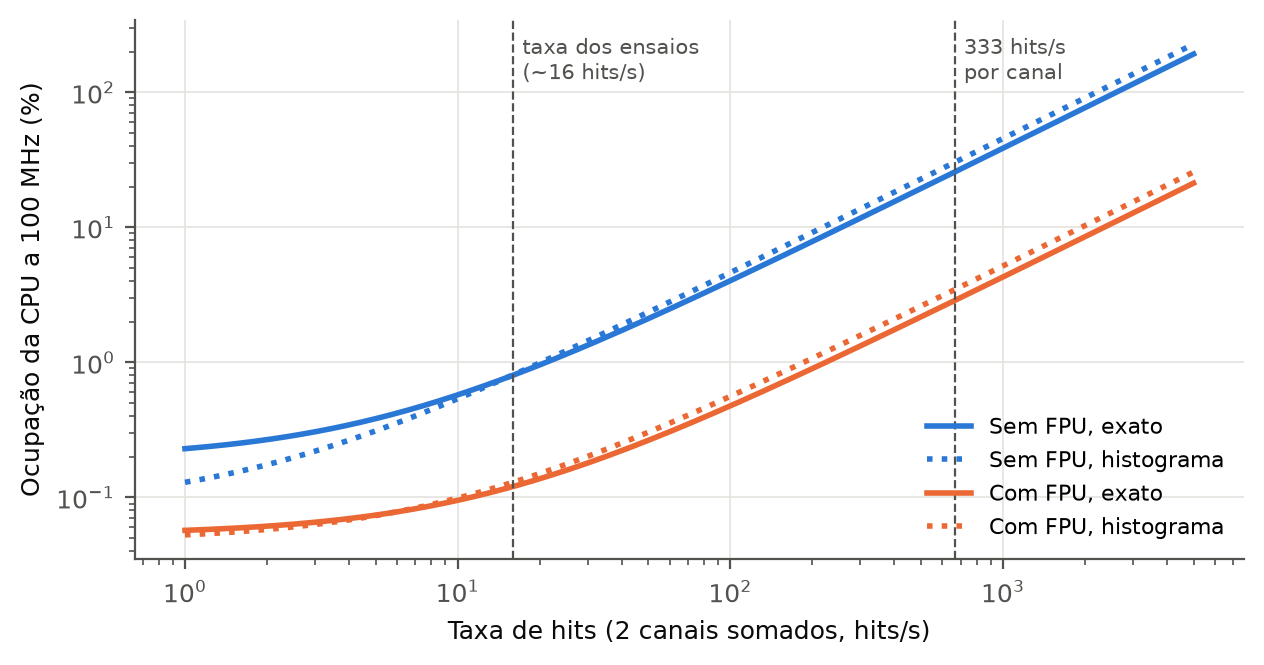
\includegraphics[width=0.85\textwidth]{figs/embarcado/fig_carga_cpu.png}
	\caption{Ocupação da CPU da MicroBlaze a 100\,MHz pela cadeia embarcada em função da taxa de \textit{hits}, extrapolada dos ciclos medidos por \textit{hit}, por fechamento de janela e pela MLP. As linhas verticais marcam a taxa dos ensaios da bomba e a maior taxa sustentada em ensaio elétrico. No modo exato, o fechamento da janela foi medido com cerca de 80 \textit{hits} e cresce como \(n \log n\); a extrapolação o subestima em taxas altas, e acima de 1\,024 \textit{hits} por canal por janela (cerca de 205 \textit{hits}/s por canal) o modo exato deixa de se aplicar.}
	\label{sim:fig:carga}
\end{figure}

\mbParagrafoCarga

A Tabela~\ref{sim:tab:memoria} resume a memória. O binário de teste da cadeia, com a MLP int8 e sem o caminho float32, ocupa de \mbTextoMin{} a \mbTextoMax\,kB de código e constantes, incluindo cerca de 10\,kB de \textit{hits} de teste que não existem no firmware real.

\begin{table}[htbp]
	\centering
	\small
	\caption{Memória da cadeia embarcada (ELF de teste, \texttt{mb-gcc} 2022.2, \texttt{-O2}).}
	\label{sim:tab:memoria}
	\begin{tabular}{lrr}
		\toprule
		\textbf{Item} & \textbf{Sem FPU} & \textbf{Com FPU} \\
		\midrule
		Código e constantes, modo exato (kB) & \mbTextoExatoSoft & \mbTextoExatoFpu \\
		Código e constantes, modo histograma (kB) & \mbTextoHistSoft & \mbTextoHistFpu \\
		Estado da janela, modo exato (kB) & 65,6 & 65,6 \\
		Estado da janela, modo histograma (kB) & 10,3 & 10,3 \\
		Pesos int8 e vieses das duas redes (kB) & \(\approx 9{,}8\) & \(\approx 9{,}8\) \\
		Pesos float32 das duas redes, se usados (kB) & \(\approx 37\) & \(\approx 37\) \\
		\bottomrule
	\end{tabular}
\end{table}

% =======================================================================================================
\subsection{Discussão}
\label{sim:sec:discussao}

\subsubsection{Qual rota usar}

A Tabela~\ref{sim:tab:rotas} reúne o custo em lógica de cada alternativa. Os números da MicroBlaze vêm da síntese do mesmo sistema usado na simulação e servem para dimensionar o acréscimo da FPU; o processador em si já existe no MOMEA e não é um custo da cadeia.

\begin{table}[htbp]
	\centering
	\small
	\caption{Recursos lógicos no XC7A35T: núcleo da MicroBlaze (síntese) e IP HLS (pós-roteamento).}
	\label{sim:tab:rotas}
	\begin{tabular}{lrrrr}
		\toprule
		\textbf{Bloco} & \textbf{LUT} & \textbf{FF} & \textbf{DSP} & \textbf{BRAM (36\,kb)} \\
		\midrule
		MicroBlaze sem FPU (núcleo) & 1\,361 & 857 & 4 & --- \\
		MicroBlaze com FPU estendida (núcleo) & 2\,322 & 1\,599 & 6 & --- \\
		Acréscimo da FPU & 961 & 742 & 2 & --- \\
		IP HLS int8 (duas redes) & 656 & 682 & 14 & 3,5 \\
		Memória local de 128\,kB (sistema simulado) & 17 & 16 & --- & 32 \\
		\bottomrule
	\end{tabular}
\end{table}

Para a aplicação atual, uma decisão a cada 5\,s, as duas rotas sobram. \mbParagrafoRota{} O IP HLS é \mbFatorHls{} vezes mais rápido que a MicroBlaze sem FPU e libera o processador, ao custo de 14 DSPs e 3,5 blocos de BRAM; ele se justificaria para classificar cada \textit{hit} em taxas altas, para modelos maiores ou se a MicroBlaze já estiver saturada pela pilha de rede. Em qualquer caso, a parte cara da cadeia não é a rede, mas o processamento por \textit{hit}, dominado pelos logaritmos; esse custo é o mesmo nas duas rotas, porque os descritores ficam no processador. Se a taxa de \textit{hits} crescer muito, o próximo passo natural é calcular na lógica as grandezas por \textit{hit} (incluindo os logaritmos, por tabela) e deixar à MicroBlaze apenas o fechamento da janela.

Entre os modos de percentis, o exato é preferível enquanto a janela couber na memória, porque preserva a decisão do modelo de referência em todas as janelas. O histograma troca cerca de 2,6\,\% de classes diferentes por memória constante e custo por \textit{hit} independente da taxa. Histogramas mais finos reduziriam essa diferença.

\subsubsection{O que a simulação garante}

A cadeia de verificação estabelece, com critérios explícitos, que: (i) a exportação do modelo e a implementação em C reproduzem o modelo de referência, bit a bit no caso int8; (ii) os descritores calculados em C a partir do registro bruto reproduzem os da Seção~\ref{sec:mm_bomba}; (iii) o RTL gerado pelo HLS é funcionalmente idêntico ao C e fecha a temporização na peça do MOMEA; e (iv) o binário compilado para a MicroBlaze produz os mesmos resultados em um processador simulado no nível RTL, com custo de tempo medido em ciclos.

A simulação não cobre, porém, o que depende da placa e do sistema completo:
\begin{itemize}
	\item a integração com o projeto atual do MOMEA, cuja ocupação de recursos não foi verificada; os recursos do IP foram obtidos fora de contexto, e o sistema MicroBlaze simulado não é o do MOMEA;
	\item o tempo de parede no firmware real, com caches ou memória externa, interrupções, recepção dos registros e pilha UDP concorrendo pelo processador;
	\item a base de tempo da janela: no treino, as janelas usaram a hora de chegada dos registros no computador; na placa, usarão o relógio local. Com o carimbo de tempo de \textit{hardware} ainda não implementado, pequenas diferenças na fronteira das janelas são esperadas;
	\item o comportamento elétrico do \textit{front-end} e do conversor, incluindo a saturação observada nos ensaios da bomba (Seção~\ref{sec:mm_bomba}).
\end{itemize}

\subsubsection{O modelo continua sendo o limite}

A implementação não muda a capacidade de generalização do modelo. Na Seção~\ref{sec:res_bomba}, a frequência generalizou para corridas não vistas (erro médio de 4 a 6\,Hz), mas a configuração das válvulas não (21 a 28\,\% de acurácia por corrida deixada de fora, para 14\,\% de acaso), e os dados têm limitações sérias: uma única corrida por condição, ordem fixa, limiar variável entre sessões e 70\,\% dos \textit{hits} saturados (Seção~\ref{sec:mm_bomba}). A contribuição deste trabalho é a infraestrutura: um fluxo que leva qualquer modelo do mesmo formato do Python ao FPGA, com verificação automática em cada nível. Retreinar com dados melhores exige apenas regenerar os cabeçalhos e repetir os testes; o código e o \textit{hardware} não mudam.

% =======================================================================================================
